% 1. ročník, hodina 66: slovní úlohy a grafy lineární/konstantní funkce.
% Model Orlíku: číselné zadání inspirováno Realisticky.cz, 020108 Lineární funkce I:
% https://www.realisticky.cz/ucebnice/01%20Matematika%20S%C5%A0/02%20Funkce%20a%20rovnice/01%20Line%C3%A1rn%C3%AD%20funkce/08%20Line%C3%A1rn%C3%AD%20funkce%20I.pdf
% Realisticky.cz uvádí 500 mil. m3, přítok 4000 m3/s, odtok 1000 m3/s, mez 780 mil. m3.
% Příběh, metodické otázky, graf, vedlejší úlohy a řešení jsou nově formulované.
% Jde o idealizovaný didaktický model, ne o předpověď bezpečnosti hráze.
\documentclass[11pt,a4paper]{article}
\input{../../sablony/pripravy/priprava.sty}
\usepackage{tikz}
\usetikzlibrary{arrows.meta}
\nastavPripravu{1. ročník}{Funkce}{66}{Slovní úlohy s lineární a konstantní funkcí}
\begin{document}
\poznamka{Časové jádro 45 min: porozumění situaci 5 min, čistý přítok a převod jednotek 9 min,
sestavení předpisů 7 min, tabulka a graf 11 min, průsečík a interpretace 8 min,
shrnutí a zadání domácí práce 5 min. Pro graf použij přiložený pracovní list.
Rezervní varianta s jiným přítokem a druhá slovní úloha jsou nad rámec jádra.}

\blok{Přehrada Orlík: dvě závislosti v jedné soustavě}
Připomeňme si rozdíl: \textbf{lineární funkce} popisuje rovnoměrnou změnu hodnoty,
zato \textbf{konstantní funkce} se s argumentem nemění. V praxi lze obě zobrazit
současně: jedna udává aktuálně modelovaný stav, druhá pevnou mez.

\begin{zadaniBox}[title={Hlavní úloha: model plnění nádrže Orlík}]
Uvažujme \emph{zjednodušený model} povodňové situace. Na počátku je v nádrži
$500$ milionů $\mathrm{m}^3$ vody. Do nádrže přitéká $4000\ \mathrm{m}^3/\mathrm{s}$
a odtéká $1000\ \mathrm{m}^3/\mathrm{s}$. Přítok i odtok považujte po celou
uvažovanou dobu za konstantní. Referenční maximální objem nádrže je
$780$ milionů $\mathrm{m}^3$.

\begin{enumerate}[label=\alph*)]
\item Určete čistý přírůstek vody za sekundu a za hodinu.
\item Zapište $V(t)$, objem vody v milionech $\mathrm{m}^3$ po $t$ hodinách.
\item Zapište konstantní funkci $K(t)$ pro referenční kapacitu.
\item Doplňte tabulku, oba grafy zakreslete do jedné soustavy a určete jejich průsečík.
\item Určete věcný definiční obor a obor hodnot plnicího modelu \emph{do dosažení kapacity}.
\end{enumerate}
\end{zadaniBox}

\blok{Od veličin k předpisům}
\begin{prikladReseniBox}[title={Řešení: čistý přítok a převod jednotek}]
Jakou změnu objemu dostaneme za sekundu, minutu a hodinu?
\tcblower
Čistý přítok je
\[
  4000-1000=3000\ \mathrm{m}^3/\mathrm{s}.
\]
Za minutu přibude $3000\cdot60=180\,000\ \mathrm{m}^3$;
za hodinu $3000\cdot3600=10\,800\,000\ \mathrm{m}^3=10{,}8$ mil. $\mathrm{m}^3$.
Proto při $t$ vyjádřeném v hodinách dostáváme
\[
  V(t)=500+10{,}8t,\qquad K(t)=780.
\]
Koeficient $10{,}8$ je směrnice v milionech $\mathrm{m}^3$ za hodinu.
Číslo $500$ je počáteční stav a hodnota $780$ je referenční mez.
\end{prikladReseniBox}

\begin{center}
\small
\begin{tabular}{@{}lrrrrr@{}}
\toprule
$t$ [h] & $0$ & $5$ & $10$ & $20$ & $24$\\
\midrule
$V(t)$ [mil. $\mathrm{m}^3$] & $500$ & $554$ & $608$ & $716$ & $759{,}2$\\
$K(t)$ [mil. $\mathrm{m}^3$] & $780$ & $780$ & $780$ & $780$ & $780$\\
\bottomrule
\end{tabular}
\end{center}

\blok{Grafické řešení a význam průsečíku}
\begin{center}
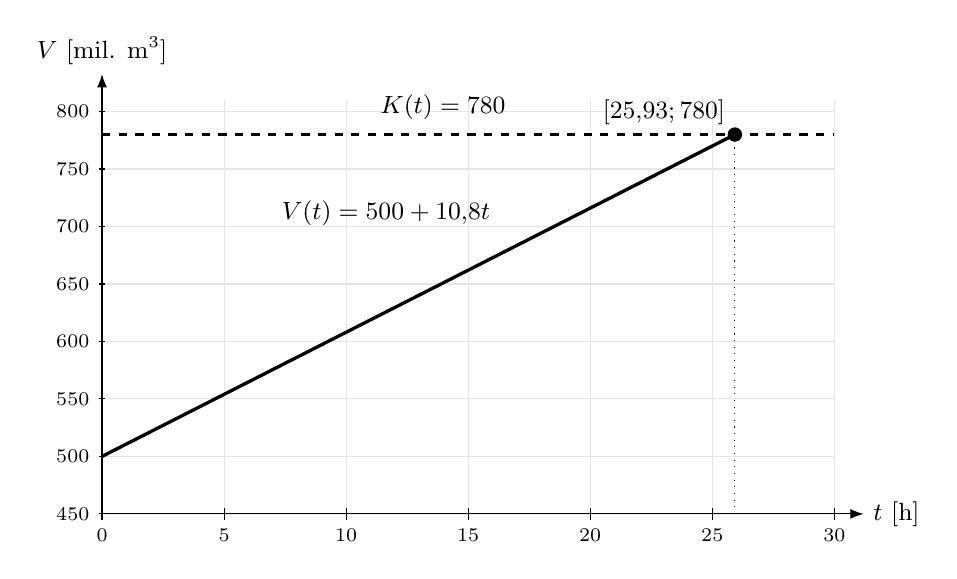
\begin{tikzpicture}[x=.31cm,y=.73cm,>=Latex]
% Souřadnice v grafu: svisle je (V - 450)/50. Osa začíná na 450, což je výslovně označeno.
\draw[step=5,gray!14,very thin] (0,0) grid (30,7);
\foreach \t in {0,5,...,30}{\draw[gray!20] (\t,0)--(\t,7.2);}
\foreach \v in {0,1,...,7}{\draw[gray!20] (0,\v)--(30,\v);}
\draw[->] (0,0)--(31.2,0) node[right,font=\small] {$t$ [h]};
\draw[->] (0,0)--(0,7.65) node[above,align=center,font=\small] {$V$ [mil. $\mathrm{m}^3$]};
\foreach \t in {0,5,...,30}{\draw (\t,.10)--(\t,-.10) node[below,font=\scriptsize] {\t};}
\foreach \v/\label in {0/450,1/500,2/550,3/600,4/650,5/700,6/750,7/800}{
  \draw (.12,\v)--(-.12,\v) node[left,font=\scriptsize] {$\label$};}
\draw[very thick] (0,1)--(25.925926,6.6);
\draw[very thick,dashed] (0,6.6)--(30,6.6);
\fill (25.925926,6.6) circle (2.6pt);
\draw[dotted] (25.925926,0)--(25.925926,6.6);
\node[above left,font=\small] at (25.925926,6.6) {$[25{,}93;780]$};
\node[font=\small,anchor=south east] at (16.3,4.85) {$V(t)=500+10{,}8t$};
\node[font=\small,anchor=south west] at (11,6.68) {$K(t)=780$};
\end{tikzpicture}
\end{center}
\poznamka{Osa objemu začíná na $450$ mil. $\mathrm{m}^3$, nikoli na nule: přibližujeme
zajímavou část grafu, včetně obou přímek. Všimni si rozdílu jednotek na osách.
Čárkovaná vodorovná přímka je modelovaná mez; nejde o skutečný časový průběh objemu.}

\begin{prikladReseniBox}[title={Řešení: okamžik dosažení meze}]
Kdy se modelovaný objem vyrovná referenční kapacitě? Uveďte také věcný obor modelu.
\tcblower
\[
  500+10{,}8t=780
  \quad\Longrightarrow\quad
  t=\frac{280}{10{,}8}=\frac{700}{27}\doteq25{,}93\ \mathrm{h}.
\]
Průsečík grafů je přibližně $[25{,}93;780]$.
Při sledování nádrže pouze \emph{do dosažení meze} volíme
\[
 D(V)=\left\langle0;\frac{700}{27}\right\rangle,\qquad
 H(V)=\langle500;780\rangle.
\]
Hodnota $V(24)=759{,}2$ znamená, že po 24 hodinách je v nádrži podle
modelu $759{,}2$ mil. $\mathrm{m}^3$. Zbývá $20{,}8$ mil. $\mathrm{m}^3$.
\end{prikladReseniBox}

\blok{Co výsledek říká a co neříká}
Funkce $V$ předpokládá neměnný přítok a odtok. Při skutečné povodni se ale obě
veličiny mění, takže nepočítáme předpověď konkrétní události. Dosažení
referenčního objemu \textbf{neznamená automaticky protržení hráze}.
To závisí na provozu vodního díla, skutečných mezních hladinách,
bezpečnostních přelivech a mnoha dalších okolnostech.

\blok{Samostatné procvičování}
\begin{zadaniReseniBox}[title={Základní otázky k modelu}]
\begin{enumerate}[label=\alph*)]
\item Za jak dlouho podle modelu vzroste objem vody o $108$ mil. $\mathrm{m}^3$?
\item Jaká je hodnota konstantní funkce $K$ při $t=7$ a co znamená její směrnice?
\item Jak se změní předpis $V(t)$, jestliže se odtok zvýší na $2000\ \mathrm{m}^3/\mathrm{s}$?
\end{enumerate}
\tcblower
\begin{enumerate}[label=\alph*)]
\item $108/10{,}8=10$ hodin; $V(10)=608$.
\item $K(7)=780$; směrnice $0$ znamená pevnou mez bez ohledu na čas.
\item Nový čistý přítok je $2000\ \mathrm{m}^3/\mathrm{s}$,
tedy $7{,}2$ mil. $\mathrm{m}^3/\mathrm{h}$. Předpis je
$V_2(t)=500+7{,}2t$. K dosažení $780$ by došlo za
$280/7{,}2\doteq38{,}89$ hodin.
\end{enumerate}
\end{zadaniReseniBox}

\blok{Volitelná rezerva: jiný typ modelu}
\begin{zadaniReseniBox}[title={Výrobní rozpočet a pevný limit}]
Výroba $n$ kusů stojí $C(n)=180n+1200$ Kč. Rozpočet je $3000$ Kč.
Určete, kolik nejvýše kusů lze vyrobit. Jaká je vhodná množina argumentů?
\tcblower
Konstantní funkce rozpočtu je $R(n)=3000$ Kč.
Rovnost $180n+1200=3000$ dává $180n=1800$, takže $n=10$.
Počet kusů je celé nezáporné číslo: $n\in\mathbb N_0$, nikoli libovolné
reálné číslo. V grafu proto přípustné body leží pouze nad celočíselnými argumenty.
\end{zadaniReseniBox}

\blok{Domácí úkol}
\begin{zadaniReseniBox}[title={Domácí procvičení}]
\begin{enumerate}[label=\alph*)]
\item V modelu Orlíku určete $V(8)$ a množství vody do dosažení meze v tomto okamžiku.
\item Uvažujte počáteční objem $550$ mil. $\mathrm{m}^3$ a stejný čistý přítok.
Napište nový předpis a spočtěte čas do referenční kapacity $780$ mil. $\mathrm{m}^3$.
\item V nádrži je $120\ \mathrm{m}^3$ vody a přitéká čistých $5\ \mathrm{m}^3/\mathrm{min}$.
Mezní objem je $200\ \mathrm{m}^3$. Sestavte lineární a konstantní funkci,
najděte průsečík a oba grafy načrtněte.
\item Popište dva důvody, proč model s konstantním přítokem nemusí platit po celou povodeň.
\item \textbf{Kurýrní dodávka:} V okamžiku zahájení sledování je dodávka na 35. kilometru
trasy. Dále jede stálou rychlostí $55\ \mathrm{km/h}$; cílový sklad leží na 255. kilometru.
Sestavte lineární funkci $S(t)$ pro polohu dodávky a konstantní funkci $C(t)$ pro
polohu skladu ($t$ v hodinách). Oba grafy zakreslete do jedné soustavy,
určete jejich průsečík a vysvětlete jeho význam. Uveďte definiční obor
modelu od zahájení sledování do příjezdu do skladu.
\end{enumerate}
\tcblower
\begin{enumerate}[label=\alph*)]
\item $V(8)=500+10{,}8\cdot8=586{,}4$ mil. $\mathrm{m}^3$;
zbývá $780-586{,}4=193{,}6$ mil. $\mathrm{m}^3$.
\item $V_3(t)=550+10{,}8t$; čas je $230/10{,}8=575/27\doteq21{,}30$ h.
\item $W(t)=120+5t$, $M(t)=200$, kde $t$ je v minutách.
Průsečík $[16;200]$ a modelová doba $0\le t\le16$ minut.
\item Například: přítok s časem kolísá; odtok reguluje provoz nádrže;
model ignoruje další přítoky, srážky nebo vodní ztráty.
\item $S(t)=35+55t$, $C(t)=255$. Z rovnice $35+55t=255$ plyne
$t=4$ h. Grafy se protínají v bodě $[4;255]$; dodávka po čtyřech hodinách
přijede do skladu. Pro sledovanou cestu volíme $D(S)=D(C)=\langle0;4\rangle$
a $H(S)=\langle35;255\rangle$, zatímco $H(C)=\{255\}$.
\end{enumerate}
\end{zadaniReseniBox}
\poznamka{Čísla hlavního příkladu pocházejí z učební modelové úlohy 2.1.8
na Realisticky.cz, nikoli ze současného měření přehrady. Ostatní slovní
úlohy jsou nové. U žáků kontroluj převody $\mathrm{m}^3/\mathrm{s}\to$ mil.
$\mathrm{m}^3/\mathrm{h}$, popis jednotek os a věcný význam průsečíku.
Opakuj, že rovnost dvou funkcí modeluje dosažení stanovené meze, nikoli fyzikální poruchu hráze.}
\end{document}
